% ====================================================================
%+
% SECTION:
%    grb.tex  % eg lenstimedelays.tex
%
% CHAPTER:
%    transients.tex  % eg cosmology.tex
%
% ELEVATOR PITCH:
%    Explain in a few sentences what the relevant discovery or
%    measurement is going to be discussed, and what will be important
%    about it. This is for the browsing reader to get a quick feel
%    for what this section is about.
%
% COMMENTS:
%
%
% BUGS:
%
%
% AUTHORS:
%    Phil Marshall (@drphilmarshall)  - put your name and GitHub username here!
%-
% ====================================================================

\section{Gamma-Ray Burst Afterglows}
\def\secname{grbs}\label{sec:\secname} % For example, replace "keyword" with "lenstimedelays"

\credit{ebellm} % (Writing team)

Gamma-ray bursts (GRBs) are relativistic explosions typically classified by the temporal duration of their initial gamma-ray emission: Long GRBs, that mark the endpoint of the lives of some massive stars, and short GRBs, believed to originate from the merger of binary neutron stars.
GRB emission is known to be beamed: the initial prompt gamma-ray emission is seen only for observers looking at the jet axis. The longer-wavelength X-ray, optical, and radio afterglow may be seen both by on- and off-axis observers.  The latter case is known as an orphan afterglow, due to the absence of gamma-ray emission.  
On- and off-axis afterglows are predicted to have different temporal
signatures in the optical: On-axis events decay as a power-law until a jet
break, while off-axis events should be fainter and show an initial rise
(Figure \ref{fig:afterglow_lcs}).
Despite systematic searches, no convincing orphan afterglow candidates have yet been discovered, limiting our knowledge of the beaming fraction of GRBs and hence their true rates.
Well-sampled orphan afterglow lightcurves would also permit study of the GRB 
jet structure.

\begin{figure}[hbt]
\centerline{
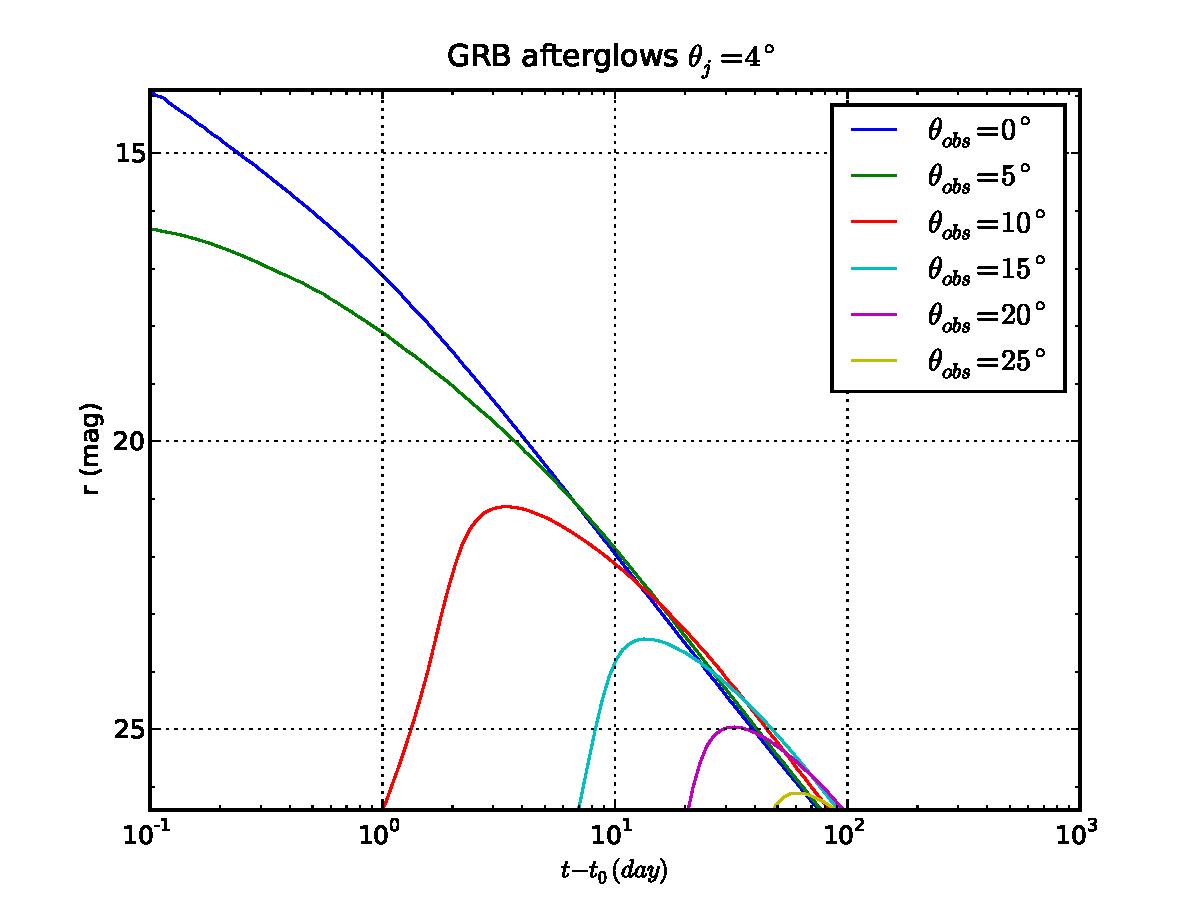
\includegraphics[width=0.6\textwidth]{figs/transients/predicted_afterglow_lcs_mag.pdf}
}
\caption{
Predicted light curves of GRB afterglows. The model of the forward shock emission is from \citealt{2002ApJ...576..120T}
(code courtesy of Alin Panaitescu). The adopted global and microphysical parameters reproduce the properties
of well observed GRBs:
jet half opening angle $\theta_j = 4^\circ$, the isotropic equivalent energy of $E_{\rm iso} = 5\times10^{53} \rm erg$,
ambient medium density $n = 1$ g cm$^{-3}$, and the slope of the electron energy distribution $\rm p = 2.1$.
The apparent $r$-band magnitudes are on the AB scale assuming a source redshift $z = 1$ and a number
of observer locations with respect to the jet axis $\theta_{\rm obs}$.
}
\label{fig:afterglow_lcs}
\end{figure}

Because of their rarity, in all but one case \citep{2015ApJ...803L..24C} to date GRBs have been discovered using their prompt emission by hard X-ray or gamma-ray all-sky monitors.  
This selection imposes biases on the population of relativistic explosions we observe.  
Baryon-loading in the GRB jet---a ``dirty fireball'' \citep{2003ApJ...591.1097R}---can lead to on-axis events without gamma-ray emission.  Only one plausible candidate has been identified to date \citep{2013ApJ...769..130C}.  
Discovery of new dirty fireballs---if distinguished from off-axis events--would clarify the rates of these events and enhance our understanding of the diversity of stellar death.

LSST is the survey most capable of resolving these decades-old questions.  Due to its large aperture and etendue, LSST can detect faint, fast-fading, and rare cosmological events, potentially enabling population studies of the high-redshift universe.  
\citet{2015A&A...578A..71G} estimated LSST could detect 50 orphan afterglows each year, more than any other planned survey.

%deep survey helps due to time dilation

%beaming fraction and true rates; jet structure; dirty fireballs?
%GRB-SN connection; probe high-z star formation?

%other fast transients: Fast transients and SN shock breakout?  flash spectroscopy

The challenge of detecting and recognizing GRB afterglows in the LSST data in 
real time makes this science case a useful proxy for other fast transient 
science cases that benefit from $N > 2$ visits per night.  In particular, this 
includes discovering supernovae soon after explosion for flash spectroscopy or 
shock breakout searches.

% need appropriate cadences to support value of realtime alert stream

% --------------------------------------------------------------------

\subsection{Target measurements and discoveries}
\label{sec:\secname:targets}

GRB afterglow discovery is among the science cases that places the greatest stress on the LSST cadence.  Because afterglows fade rapidly---dropping several magnitudes in the first few hours---high cadence observations are required to detect the fast fading.  
If an afterglow candidate can be recognized in real time, it will be possible to trigger TOO spectroscopy (to measure a redshift and confirm the event is cosmological), X-ray and radio observations (to detect a high-energy counterpart and the presence of a jet), and additional photometry (to characterize the lightcurve evolution).  If there is no source at the location of the transient in the coadded reference image, two consecutive observations in the same filter separated by an hour or two are the minimum required to potentially trigger followup of a fast-fading event.  
However, a third or fourth observation in a single night---ideally in the same filter---would improve the purity of the sample.  Observations in other bands at high cadence are less useful because they require assumptions about the event's SED and its evolution to determine if a source is truly fading.

Distinguishing orphan afterglows from on-axis events (whether conventional GRBs or dirty fireballs) will also require more than two detections.  Orphan events may prove harder to recognize in real time, because they are intrinsically fainter than on-axis events and show an initial rise rather than a rapid decay.  
Additionally, because of relativistic time dilation high redshift events are easier to detect, but these events will be fainter and more difficult to follow up.
Accordingly, population studies of orphan afterglow candidates may be best conducted with LSST photometry alone.  These may only be productive if LSST has suffiently frequent revisits to a field in a single filter.

% --------------------------------------------------------------------

\subsection{Metrics}
\label{sec:\secname:metrics}

The core figure of merit for GRB afterglows is simply the raw number of on- and off-axis events detectable in two, three, or more observations, preferably in a single filter.

The appropriate way to derive these detections is to conduct a Monte Carlo simulation of a cosmological population of GRBs and fold it through the LSST observing cadence \citep[cf.][]{2011PASP..123.1034J}.  We are developing this infrastructure for the MAF framework.  

In the meantime, simplified metrics can give us a general idea of how well a given cadence can characterize fast-evolving transients such as GRBs.
The \texttt{TransientMetric} and \texttt{TripletBandMetric} 
can give us a clue.  We have created a new metric, \texttt{GRBOnAxisMetric}, that replaces the linearly rising and decaying lightcurve in 
\texttt{TransientMetric} with the $F \sim t^{-\alpha}$ decay characteristic of on-axis afterglows.  (For the time being, we neglect the jet break that steepens the rate of decay; this implies that our detectability estimates are optimistic.)

We simulate random on-axis afterglows using the parameters of \citet{2011PASP..123.1034J}: the R-band apparent magnitude at 1 minute after explosion is randomly drawn from a Gaussian with $\mu=15.35$, $\sigma=1.59$ and decays with $\alpha=1.0$.  For these quick estimates we simply assume zero color difference between in all LSST bands.

\textbf{how long are these above limiting magnitude at these pars? feed into TripletBandMetric, or controltime...}

%Can use https://github.com/lsst/sims_maf/blob/master/python/lsst/sims/maf/metrics/tgaps.py or https://github.com/lsst/sims_maf/blob/master/python/lsst/sims/maf/metrics/cadenceMetrics.py (Inter/Intra-night) to get histograms.  Would be nice to extend to single-band, N-offset

% --------------------------------------------------------------------

\subsection{OpSim Analysis}
\label{sec:\secname:analysis}

OpSim analysis: how good would the default observing strategy be, at
the time of writing for this science project?


% --------------------------------------------------------------------

\subsection{Discussion}
\label{sec:\secname:discussion}

Discussion: what risks have been identified? What suggestions could be
made to improve this science project's figure of merit, and mitigate
the identified risks?


% ====================================================================

\navigationbar
